\documentclass[journal=jcim,manuscript=applicationnotes]{achemso}


%%%%%%%%%%%%%%%%%%%%%%%%%%%%%%%%%%%%%%%%%%%%%%%%%%%%%%%%%%%%%%%%%%%%%
%% Place any additional packages needed here.  Only include packages
%% which are essential, to avoid problems later. Do NOT use any
%% packages which require e-TeX (for example etoolbox): the e-TeX
%% extensions are not currently available on the ACS conversion
%% servers.
%%%%%%%%%%%%%%%%%%%%%%%%%%%%%%%%%%%%%%%%%%%%%%%%%%%%%%%%%%%%%%%%%%%%%
\usepackage[version=3]{mhchem} % Formula subscripts using \ce{}
\usepackage{subcaption}
\usepackage{array}
\usepackage{url}
\usepackage{xr}
%\usepackage{xr-hyper}
\usepackage{hyperref}
\usepackage{multirow}
\usepackage{listings}
\usepackage[finalizecache,cachedir=.]{minted}
\usepackage[flushleft]{threeparttable}
%\captionsetup[figure]{font=small,labelfont=small}

\lstset{
breaklines=true,
breakatwhitespace=true,
captionpos=b,
frame=single
}


\makeatletter
\newcommand*{\addFileDependency}[1]{% argument=file name and extension
  \typeout{(#1)}
  \@addtofilelist{#1}
  \IfFileExists{#1}{}{\typeout{No file #1.}}
}
\setlength\acs@tocentry@height{8.25cm}
\setlength\acs@tocentry@width{4.45cm}
\makeatother
\newcommand*{\myexternaldocument}[1]{%
    \externaldocument{#1}%
    \addFileDependency{#1.tex}%
    \addFileDependency{#1.aux}%
}

\myexternaldocument{supplement}
\newcommand*\mycommand[1]{\texttt{\emph{#1}}}

\setkeys{acs}{maxauthors = 0}

\title{SolTranNet -- A machine learning tool for fast aqueous solubility prediction.}
\keywords{deep learning, machine learning, molecular property prediction, solubility, tool}
\author{Paul G. Francoeur}
\email{paf46@pitt.edu}
\author{David R. Koes}
\affiliation[Pitt]{Department of Computational and Systems Biology, University of Pittsburgh, Pittsburgh, PA 15260}

\begin{document}

\begin{tocentry}

% Some journals require a graphical entry for the Table of Contents.
% This should be laid out ``print ready'' so that the sizing of the
% text is correct.

% Inside the \texttt{tocentry} environment, the font used is Helvetica
% 8\,pt, as required by \emph{Journal of the American Chemical
% Society}.

% The surrounding frame is 9\,cm by 3.5\,cm, which is the maximum
% permitted for  \emph{Journal of the American Chemical Society}
% graphical table of content entries. The box will not resize if the
% content is too big: instead it will overflow the edge of the box.

% This box and the associated title will always be printed on a
% separate page at the end of the document.
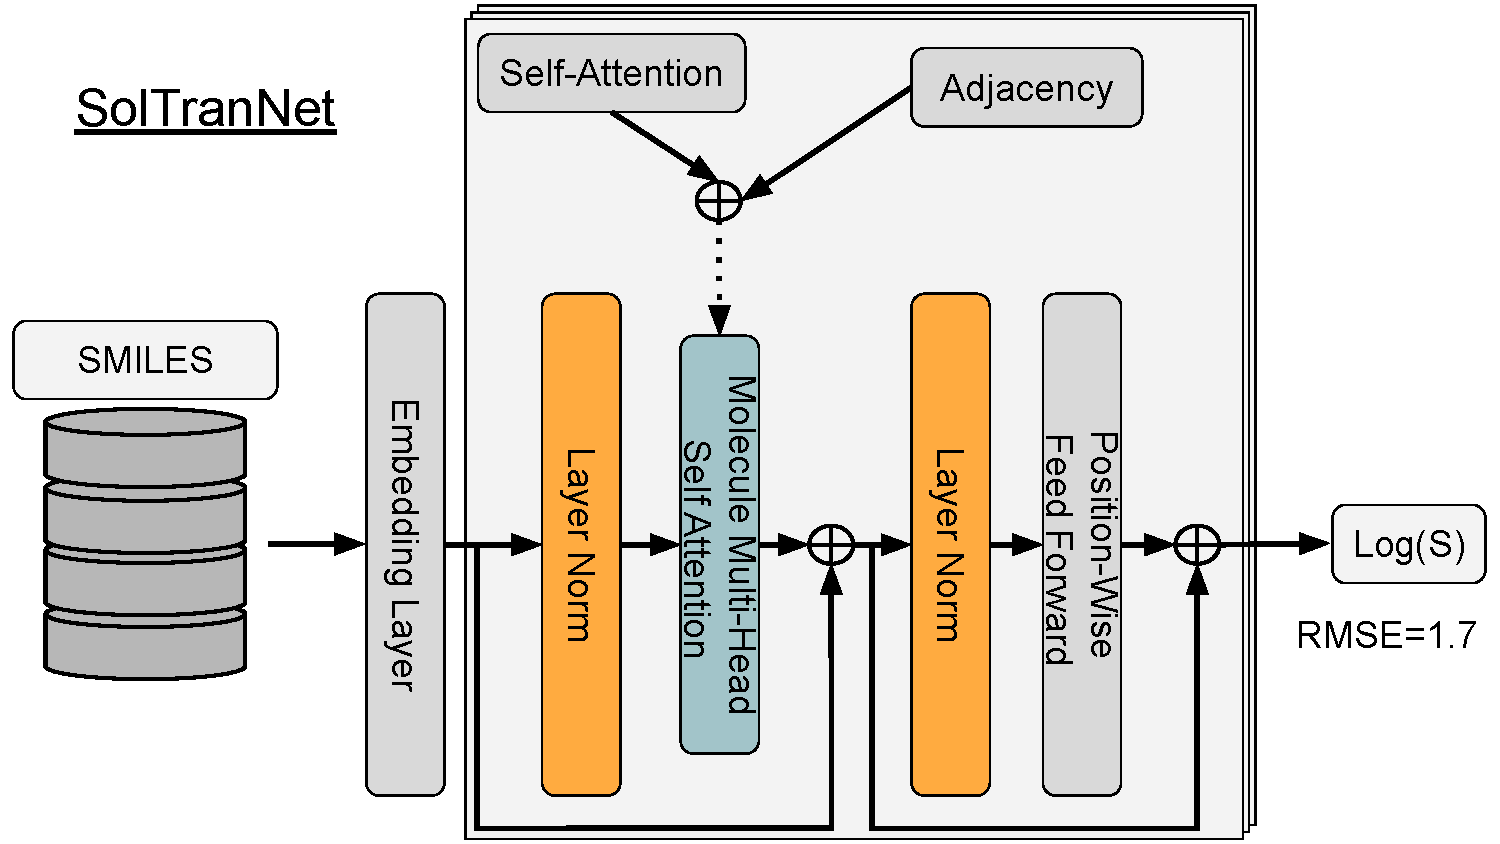
\includegraphics[width=\linewidth]{figures/TOC_soltrannet.pdf}
\end{tocentry}

%%%%%%%%%%%%%%%%%%%%%%%%%%%%%%%%%%%%%%%%%%%%%%%%%%%%%%%%%%%%%%%%%%%%%
%% The abstract environment will automatically gobble the contents
%% if an abstract is not used by the target journal.
%%%%%%%%%%%%%%%%%%%%%%%%%%%%%%%%%%%%%%%%%%%%%%%%%%%%%%%%%%%%%%%%%%%%%
\begin{abstract}
While accurate prediction of aqueous solubility remains a challenge in drug discovery, machine learning (ML) approaches have become increasingly popular for this task.
For instance, in the Second Challenge to Predict Aqueous Solubility (SC2), all groups utilized machine learning methods in their submissions.
We present SolTranNet, a molecule attention transformer to predict aqueous solubility from a molecule's SMILES representation.
Atypically, we demonstrate that larger models perform worse at this task, with SolTranNet's final architecture having 3,393 parameters while outperforming linear ML approaches.
SolTranNet has a three-fold scaffold split cross-validation root mean square error (RMSE) of 1.459 on AqSolDB and a RMSE of 1.711 on a withheld test set.
We also demonstrate that, when used as a classifier to filter out insoluble compounds, SolTranNet achieves a sensitivity of 94.8\% on the SC2 dataset and is competitive with the other methods submitted to the competition.
SolTranNet is distributed via \textsc{pip}, and its source code is available at \url{https://github.com/gnina/SolTranNet}.

\end{abstract}

%%%%%%%%%%%%%%%%%%%%%%%%%%%%%%%%%

%%%%%%%%%%%%%%%%%%%%%%%%%%%%%%%%%%%%%%%%%%%%%%%%%%%%%%%%%%%%%%%%%%%%%
%% Introduction and Background
%%%%%%%%%%%%%%%%%%%%%%%%%%%%%%%%%%%%%%%%%%%%%%%%%%%%%%%%%%%%%%%%%%%%%
\section{Introduction}
Aqueous solubility is an important physicochemical property for drug discovery, in part due to humans being 60\% water\cite{HumanWater} and water being the primary solvent in most assays. 
Besides absorption into the body, a drug's behavior in water is linked to its distribution and elimination in the body.
Consequently, lack of aqueous solubility can potentially result in failure throughout the drug discovery pipeline.\cite{LIPINSKI1997,DI2006446,EKINS2002305}
Ideally, one would directly measure the solubility of a given compound.
However, such an approach is slow, expensive, and requires the compound to be available for experiments.
With the increasing size of molecular screening libraries, up to 350 million compounds,\cite{NatureVS} experimentally measuring the solubility of each compound becomes infeasible.
Thus there is a need for fast and accurate solubility prediction as an accessory to large-scale virtual screening.

Predicting aqueous solubility for a given molecule is typically performed with one of three methods: molecular simulation, quantum calculations, or an empirically fit function.
Molecular simulation approaches utilize statistical mechanics and either directly calculate the solubility from the chemical potentials of the solute and water\cite{denseStates}, or directly simulate the solute in explicit water molecules.
For direct simulation of the solute there are several methods available, as reviewed by\citet{solrev1}, which all use a large amount of computing power, and in the case of direct simulation also require a long time to reach equilibrium.

Quantum mechanics (QM) based approaches operate at a higher level of theory than simulation and are divided into two broad categories based on if the solvent is included in the calculation. 
Full QM methods include the water molecules in their calculations and are based on density functional theory\cite{solrev1}.
This approach is the most rigorous, yet suffers from underestimating the equilibrium density of the solute\cite{solrev1}, and requires the most computing power.
The other approach, continuum solvent methods, treat the water as a bulk dielectric.
This saves on computing power, but does not sample the water's degrees of freedom and assumes that the solute's charge is entirely contained in the cavity it creates in the solvent.

Both of the previous methods require a large amount of computing power in order to perform their calculations.
In order to avoid this, there has been extensive work in developing empirical models for solubility prediction\cite{solrev1,solrev2}.
These methods utilize some set of molecules with known solubility as training data and then fit a function based on features of said molecules to predict solubility.
This approach is much faster but fails to generalize to molecules outside of scope of the training set.
As in many other applications, non-parametric machine learning (ML) approaches have been supplanting traditional function fitting for this empirical approach.
Indeed, all of the approaches in the Second Challenge to Predict Aqueous Solubility (SC2) utilized ML algorithms.\cite{llinas}
\citet{boobier} showed typical ML algorithms performed equally as well as human experts for predicting the solubility of drug-like compounds.
\citet{lovric} performed a study of several ML methods, and showed that simpler ML approaches generalized better to unseen data.
Lastly, \citet{cui} showed deeper models can succeed at this task, with their 20-layer ResNet architecture.

\citet{MAT} developed the molecule attention transformer (MAT) architecture, which is modeled after the current state of the art transformer architecture for natural language processing tasks.
MAT functions by applying self-attention to a molecular graph representation of the molecule, where each node is characterized by a feature vector as described in Table~\ref{tab:atomembed}.
This feature vector is combined with an adjacency matrix describing the connectivity of the molecule and a distance matrix that describes how far apart each atom is from each other atom in a generated 3D conformer of the molecule.
The authors utilized MAT for a variety of molecular property prediction tasks, and performed well at solubility prediction without optimizing for this task.

While ML approaches have become more common for predicting aqueous solubility, there is still a lack of readily available tools.
Extensive code bases, such as DeepChem\cite{deepchem} and Chemprop\cite{chemprop}, contain training data and support for predicting aqueous solubility, but it remains the burden of the user to train new models if they wish to use the software.
Similarly, while there were 37 participants in SC2, the provided information is not enough to recreate the models that were used to generate their predictions.
For example, we know the general architecture (e.g. artificial neural networks) and training data that a particular submitter used, but do not know the hyperparameters of the architecture, nor how long the model was trained.
As such, there is an unmet need for a ML based solubility predictor that is easy to deploy and use.

Here we present SolTranNet, a ML model based on the MAT architecture, for predicting aqueous solubility.
We trained SolTranNet utilizing the SMILES and reported solubilities in AqSolDB\cite{AqSol}, as it was the largest publicly available curated set, and optimized SolTranNet for speed and quality of prediction.
SolTranNet has 0.6764 $R^2$ and 1.459 root mean square error (RMSE) on clustered cross-validation scaffold-based splits of AqSolDB, and 0.577 $R^2$ and 1.711 RMSE on our withheld test set when trained on all of AqSolDB.
We also compare to other recently published ML models.\cite{lovric,cui,boobier,llinas}
SolTranNet is available via \textsc{pip} installation for \textsc{python3}, and the source code is available at \url{https://github.com/gnina/SolTranNet}. The datasets and scripts used for this paper are available at \url{https://github.com/francoep/SolTranNet_paper}.


%%%%%%%%%%%%%%%%%%%%%%%%%%%%%%%%%%%%%%%%%%%%%%%%%%%%%%%%%%%%%%%%%%%%%
%% Methods
%%%%%%%%%%%%%%%%%%%%%%%%%%%%%%%%%%%%%%%%%%%%%%%%%%%%%%%%%%%%%%%%%%%%%
\section{Methods}

Here we describe the installation process of SolTranNet, as well as its command line and Python API.
We also describe the dataset and hyperparameter sweep utilized to fit and select the final architecture of SolTranNet.
Additionally, we describe the 4 external datasets we used to validate SolTranNet's performance against current methods.

\subsection{Installation and Usage}
We aim for SolTranNet to be easy to incorporate into a virtual screening pipeline.
As such, we have made the entire package \textsc{\textsc{pip}} installable for \textsc{python3}, which will allow for both a command line utility and usage in a \textsc{python3} environment. 
SolTranNet's dependencies are RDKit\cite{rdkit} (2017.09.1+),  NumPy\cite{numpy} (1.19.3), PyTorch\cite{pytorch} (1.7.0+), and pathlib (1.0+).
SolTranNet also supports CUDA enabled GPU acceleration via automatic detection through PyTorch.  Installation is done through \textsc{pip}: \\
        \begin{lstlisting}[frame=none,language=bash]
 python3 -m pip install soltrannet
        \end{lstlisting}
which installs a standalone command line utility:
        \begin{lstlisting}[frame=none,language=bash]
soltrannet mysmiles.txt predictions.txt
        \end{lstlisting}
as well as a Python module:
        \begin{minted}[fontsize=\footnotesize]{python}
        >>> import soltrannet as stn
        >>> predictions = list(stn.predict(["c1ccccc1","Cn1cnc2n(C)c(=O)n(C)c(=O)c12"]))
        \end{minted}
 for embedding in user defined scripts.

\subsection{Datasets}
AqSolDB\cite{AqSol} is the dataset we utilized for training SolTranNet, as it was the largest publicly available set.
AqSolDB spans a wide range of solubility values (Fig~\ref{fig:esol_hist}) and is collated from differing datasets, most of which controlled for temperature.
Notably, during this collation process, AqSolDB only screened for identical molecules, and did not verify if the solubility measurements in its datasets were measured in buffered conditions, water, or at what pH the measurement was taken.
This is especially noteworthy as differing these conditions can change the measurement by orders of magnitude.  However, an expansive solubility dataset controlled for all these factors is not currently available.
Additionally, from our previous work\cite{cd2020}, we have observed that neural network models tend to perform better with larger datasets, even if the data contains more noise.
Thus, we elected to utilize AqSolDB for our training set over the smaller ESOL\cite{esol} which was used in the original MAT publication\cite{MAT}, a comparative analysis of which can be found in Fig~\ref{fig:stndepesol}-\ref{fig:stnesolaqsol} and Table~\ref{tab:esolaqsol}.
Notably, while there are many other features available in AqsolDB, we only utilized the included SMILES strings and the reported solubilities (logS, S in mol/L).
We then utilized RDkit\cite{rdkit} to calculate the Murcko scaffolds of the molecules, in order to cluster the molecules and generate a 3-fold clustered cross-validation (CCV) split of the data.
We additionally created a withheld test set out of the molecules present in the SC2 test sets \cite{llinas} and FreeSolv \cite{freesolv}, such that no molecule in the withheld test set has an RDkit fingerprint similarity of greater than or equal to 0.9 to any molecule in AqSolDB.
The histograms of solubility values for each fold of the scaffold split, the full AqSolDB, and our withheld set are shown in Fig~\ref{fig:solhists}.
These sets were utilized to optimize SolTranNet's final architecture, as described in the Model Optimization subsection.

While the datasets described above allow for an evaluation of SolTranNet, we also seek to compare to other published models.
Thus, we also evaluate SolTranNet using previously published training and test sets.
\citet{boobier} provided a training and testing set (75 and 25 molecules respectively) in 2017 that showed a multi-layer perceptron performing equally as well as human experts.
\citet{cui} provided a training set of 9943 molecules and a testing set of 62 molecules that they utilized to evaluate a 20-layer ResNet based ML model.
\citet{lovric} provided a set of 829 molecules which they randomly split into a training, validation, and testing set consisting of 64\%, 16\%, and 20\% of the molecules respectively and evaluated the performance of random forest, light gradient boosting method, and LASSO and partial least squares regression models.
Lastly, \citet{llinas} hosted the SC2, wherein two test sets were provided and participants could utilize any training set they desired, provided that no molecule was present in the test sets.
As such, we filtered AqSolDB such that there was no overlap with any molecule present in the SC2 test set (determined by identical RDkit fingerprints) to use as a new training set.

\subsection{Model Optimization}
The general architecture of the MAT model is provided in Figure~\ref{fig:architecture}.
In order to optimize the hyperparameters for SolTranNet, we utilized a 2 stage optimization procedure (Table~\ref{tab:wandsweep}).
All hyperparameter optimizations were performed utilizing the Weights and Biases platform\cite{wandb}.
The first stage was a Bayesian with hyperband stopping criteria search over hyperparameters related to the model optimizer (Figure~\ref{tab:initsweep}). 
The objective of this search was to minimize the RMSE of the test set for the first fold of the CCV scaffold split of AqSolDB.
This resulted in the selection of the Huber loss function, the stochastic gradient descent (SGD) optimizer with momentum of 0.06, no weight decay, and a learning rate of 0.04.
We then performed a grid search over the hyperparameters describing the SolTranNet architecture for 100 epochs over each fold of the CCV scaffold split of AqSolDB (Figure~\ref{tab:archsweep}).
We additionally evaluated the first 10 models of this search with both 2D and 3D distance matrices, after which only the 2D versions of the models were evaluated for the remainder of the sweep.
During the grid search, we evaluated one model for each combination of hyperparameters.
In order to provide a point of comparison, we evaluated 4 linear ML models on each fold of the scaffold split of AqSolDB and the full AqSolDB.
These linear models are LASSO, Elastic Net, partial least squares, and ridge regression.
Each was implemented through scikit-learn\cite{scikit-learn}, and trained on bit size 2040 RDKit fingerprints for a maximum of 100,000 iterations.

\begin{figure}[tb]
    \centering
    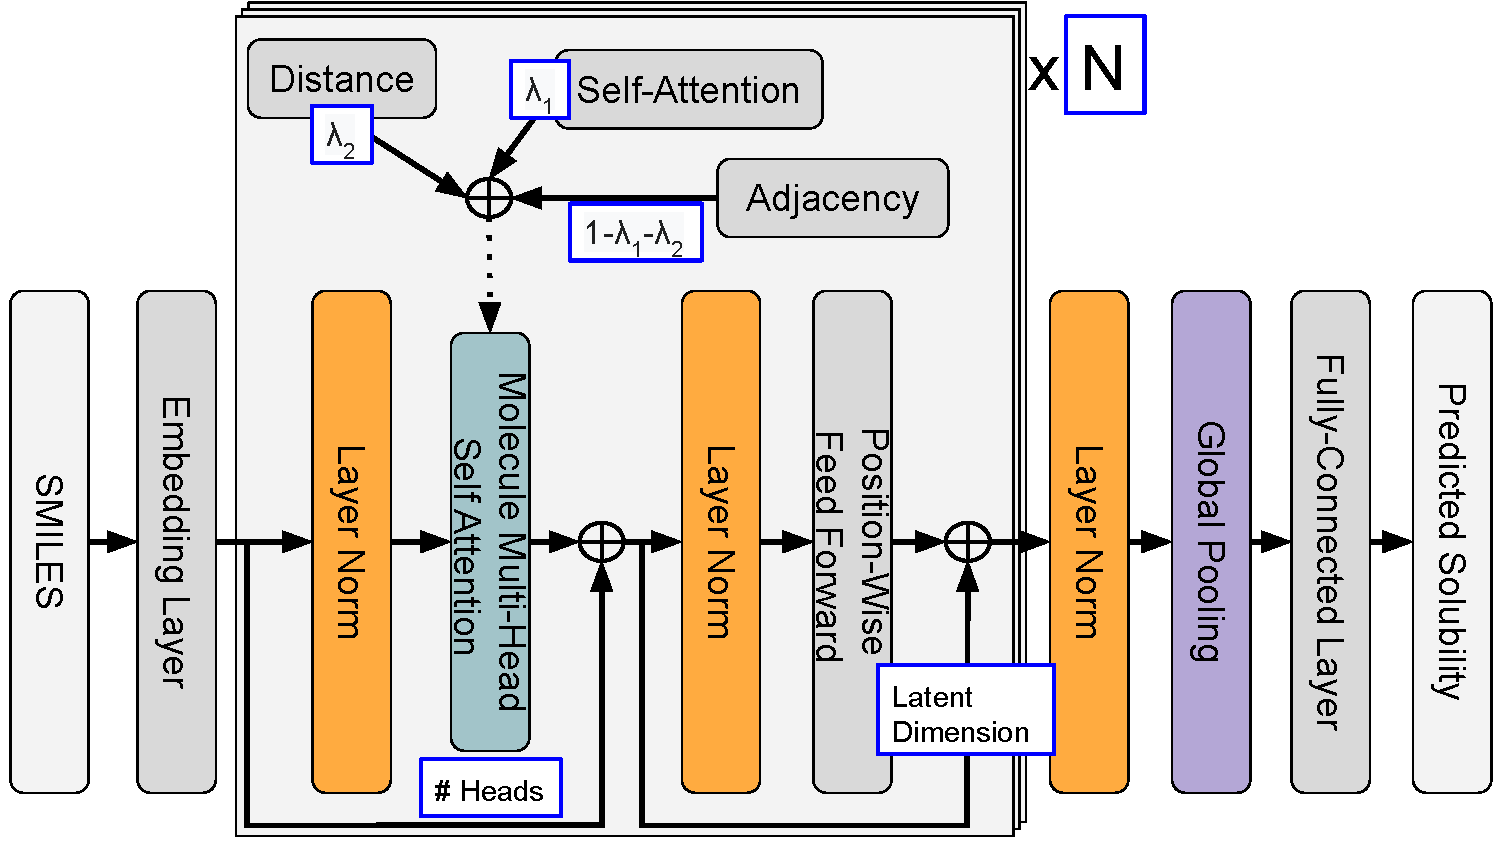
\includegraphics[width=0.7\linewidth]{figures/soltrannet_architecture.pdf}
    \caption{General Architecture of SolTranNet. Each item in a blue box is a tuned hyperparameter, whose values were tested as shown in Figure~\ref{tab:archsweep}.}
    \label{fig:architecture}
\end{figure}

In order to select the best performing model, we calculated the $R^2$ and the root mean square error (RMSE) of the predicted solubility.
Since the solubility values in AqSolDB span several orders of magnitude, the $R^2$ correlation metric is easier to perform well on.
Thus, we selected our best performing model by its RMSE performance on our withheld test set (Table~\ref{tab:solsearchrmse}).
Additionally, as we intend for this tool to be deployed for use very large datasets, we took into account the speed of SolTranNet in evaluating the results of our hyperparameter search. 

\subsection{Final model training}
The final architecture of SolTranNet utilized the following hyperparameters: 0.1 dropout, 0 lambda distance, 0.5 lambda attention, 2 attention heads, a hidden dimension of size 8, and 8 stacks in the transformer encoding layer. 
A 2D molecular representation was selected because it provided statistically equivalent results to 3D representations (Figure~\ref{fig:2dv3d}) without the computational burden of generating a 3D conformation or computing a distance matrix.
The molecular embedding layer was unchanged from the initial MAT implementation\cite{MAT} where each atom is represented as a node with a feature vector as shown in Fig~\ref{tab:atomembed}.
We also note that our molecular embedding layer calculates the features for the molecular graph from the RDKit's molecule object of each SMILES, which ensures consistency of results across different SMILES representations.
In order to select the final deployed model, we trained 5 models with different random seeds on all of AqSolDB utilizing the Huber loss function, the SGD optimizer with momentum of 0.06, no weight decay, and a learning rate of 0.04.
We dynamically stopped training after performance on the training set stopped improving for 8 epochs.
After which we selected the model architecture with the best average RMSE performance on our withheld test set and selected the best performing model from within that architecture class (Fig~\ref{fig:dynsweep}).
The dropout in the final model and our early stopping criteria both help to prevent overtraining of the deployed SolTranNet.

%%%%%%%%%%%%%%%%%%%%%%%%%%%%%%%%%%%%%%%%%%%%%%%%%%%%%%%%%%%%%%%%%%%%%
%% Results
%%%%%%%%%%%%%%%%%%%%%%%%%%%%%%%%%%%%%%%%%%%%%%%%%%%%%%%%%%%%%%%%%%%%%
\section{Results}

We first show a sampling of results of the hyperparameter sweep for the SolTranNet architecture.
We then show the speed benefit of using 2D conformers to process the SMILES string input without a loss of prediction performance.
We also analyze the effect of rare atom types on the efficacy of SolTranNet.
Lastly, we compare SolTranNet to a variety of other published ML-based solubility models.

\subsection{Selecting the Final Architecture}

To determine the final architecture of SolTranNet, we performed the two stage hyperparameter search as described in Methods.
Table~\ref{tab:solsearchrmse} shows the RMSE performance of several models from the search on the 3 fold scaffold split of AqSolDB.
We selected the top RMSE performers of each class of models (by number of parameters) to show.
Note that only a single model was evaluated for each combination of hyperparameters.
Contrary to expectation, we find that models with fewer parameters tended to perform better at solubility prediction for AqSolDB.
This was driven by better performance on Fold1.
It is the most challenging split because the distribution of solubilities in the test set is distinct from the training set (Fig~\ref{fig:solhists}).
We focus on the RMSE metric, since the large range of true solubilities makes it easier to achieve a higher Pearson $R^2$ (Table~\ref{tab:solsearchr2}).

We quantified SolTranNet's generalization by training 5 different models on all of AqSolDB and testing them on our withheld set (Table~\ref{tab:deployed}).
An ensemble of 5 models outperforms the mean of said models, but fails to beat the best performing seed (Figure~\ref{fig:dynsweep}).
As we desire SolTranNet to be as fast as possible, we elected to deploy a single model with the best performing seed.

\subsection{Conformer Generation}

SolTranNet first creates the molecular graph representation for each input molecule's SMILES.
Part of this representation is the calculation of the distance matrix, which stores the distance between each pair of atoms.
In MAT's implementation this matrix is calculated from a 3D conformer of the molecule generated by RDkit, which can be a costly process.
A much computationally cheaper process would be to utilize a 2D conformer of the molecule generated by RDkit, which is the behavior of the original MAT code if a given 3D conformer could not be computed.
We show that using a 2D or 3D conformer does not have a statistically significant difference on RMSE or $R^2$ for the first 10 hyper-parameter combinations of SolTranNet during the architecture sweep ($p=0.144$) (Figure~\ref{fig:2dv3d}).
Thus, we used distances determined via RDKit's Compute2DCoords function with default parameters as the 2D conformer for the remainder of the sweep. 
Since the final architecture does not use distance information ($\lambda_2 = 0$), distance matrix calculation is skipped, accelerating predictions.

\subsection{Salts and Rare Atom Types}
In AqSolDB, salts are explicitly represented and consist of about 11\% of the data.
Additionally 9.87\% of the AqSolDB molecules contain atoms that are typed as ``Other'' (i.e. not B, N, C, O, F, P, S, Cl, Br, or I) by SolTranNet.
These two groups overlap by 75.2\% and 83.9\% respectively; that is, unusual atom types are typically due to salts, typically in the counter ion.
Thus, we investigate the effect of fragmenting salts (by keeping the largest component, thus removing the counter ion) and removing successively larger molecules with ``Other'' typed atoms from the training data (Figure~\ref{fig:saltfragrmse},\ref{fig:saltfragr2}) in order to gain an understanding of the effect rare atom types have on model performance.
For all comparisons between identical test sets, there is no statistically significant difference between training on the full salt or the fragmented salt for the RMSE evaluations.
We note that when removing molecules containing any ``Other'' typed atom, training on fragmented salts performed better for the $R^2$ evaluation when testing with fragmented salts without losing performance on testing with normal salts (Figure~\ref{fig:noothersdf2}).
We train on the full salt since it allows less preprocessing for the user.
Additionally, removing more ``Other'' typed molecules from the training and testing data results in performance gains, as expected.
Since these ``Other'' typed atoms are potentially encountered during drug discovery, we kept them in SolTranNet's training set, but have these molecules raise a warning.

\subsection{Run-time Performance}

To benchmark SolTranNet, we determined the mean time for a solubility prediction from SMILES strings for 1,000 molecules (repeats of the 132 SC2 molecules).
Table~\ref{tab:timings} shows the mean and standard deviation of 10 runs performed with a Nvidia Titan-XP graphics card, and using 1 core of an Intel(R) Core(TM) i7-4930K CPU.
For the original MAT implementation, utilizing 3D conformer generation takes 34 times longer than 2D conformer generation on GPU (5 times longer on CPU).
SolTranNet, with fewer parameters and skipping conformer generation, runs 2.3 times faster on GPU (12.0 times faster on CPU) than MAT utilizing the 2D conformer generation.
Additionally, by implementing multiprocessing and running on a single GPU and 12 CPU cores, we are able predict 1 million molecules in 8.5 minutes.

\begin{table}
    %\centering
    \begin{tabular}{|c|l|l|}
        \hline
        \multirow{2}{*}{Model}    & \multicolumn{2}{c|}{Mean Time (std) [s/mol]} \\ 
        \cline{2-3}
          &  GPU & CPU \\
         \hline
         MAT 3D & 0.1247 (0.002075) & 0.1501 (0.001071) \\
         MAT 2D & 0.003638 (0.00039) & 0.02834 (0.001317) \\
         STN 1 CPU & 0.001583 (0.000004) & 0.002352 (0.000033)\\
         STN 12 CPU & 0.001058 (0.000019) & 0.001484 (0.000027)\\
         \hline
    \end{tabular}
    \caption{Mean time for the model to predict solubility for the original MAT implementation and SolTranNet (STN). The predictions were for 1,000 molecules consisting of repeats of the SC2 dataset. We report the mean and standard deviation (in parenthesis) of 10 runs for each model in seconds per molecule. All predictions were performed on a machine with a Nvidia Titan-XP graphics card, and an Intel(R) Core(TM) i7-4930K CPU, with a batch size of 32.}
    \label{tab:timings}
\end{table}


\subsection{SolTranNet Performance on Other Datasets}

In order to compare SolTranNet to other methods, we first verified SolTranNet's performance on ESOL\cite{esol} as in the MAT publication\cite{MAT}, and then evaluated SolTranNet on four recently published solubility training and testing sets\cite{lovric,boobier,cui,llinas} (Table~\ref{tab:othersetsrmse},\ref{tab:othersetsr2}).
To provide fair comparisons, we evaluate models trained with the provided training and testing data, and the deployed version of SolTranNet (trained on AqSolDB).
For each comparison we initially trained five models with the same dynamic stopping criteria as our training.
However, for the datasets provided by ESOL\cite{esol}, \citet{lovric}, and \citet{boobier}, this performed poorly and stopped training early due to their smaller size  (1128, 530 and 75 molecules respectively) as compared to our AqSolDB training sets (6655 CCV and 9982 full).
As such, we trained new models for 1000, 1000, and 500 epochs respectively for those sets.
Reassuringly, our implementation of the original MAT architecture and SolTranNet exhibit no statistically significant difference in performance when training with the provided ESOL random splits (p=0.073 and p=0.26 respectively).
Notably, the deployed version of SolTranNet has much worse performance on the ESOL splits ($RMSE=2.99$), but maintains a high correlation ($R^2=0.890$).
See Supplemental Table~\ref{tab:esolaqsol} for further analysis.
For the datasets provided by \citet{cui}, \citet{lovric}, and \citet{boobier}, SolTranNet's best performing model trained on the provided datasets achieves similar results to the method reported in the respective paper.
However, for the SC2 data\cite{llinas}, SolTranNet has much worse performance than the top submitted method and ranks in the lower quarter of the submitted methods.

\begin{table}
    \centering
    \begin{tabular}{|c|c|c|c|c|c|}
        \hline
        Dataset &  Reported & Training &  Best & Deployed & Overlap \\
        \hline
        ESOL MAT & 0.278 (0.20) & 0.306 (0.027) & -- & -- & 1128/1128 \\
        ESOL STN & 0.278 (0.20) & 0.289 (0.011) & -- & 2.99 (0.108) & 1119/1128 \\
        \hline
        Cui2020 & 0.681 & 0.860 (0.215) & 0.624 & 0.813 & 0/62 \\
        Boobier2017 & 0.985 & 1.274 (0.178) & 1.010 & 0.845 & 23/25 \\
        Lovric2020 & 0.720 & 0.898 (0.101) & 0.720 & 0.854 (0.0672) & 151.4/166 \\
        Llinas2020 set1 & 0.780 & 1.119 (0.163) & 0.952 & 1.004 & 79/100 \\
        Llinas2020 set2 & 1.060 & 1.811 (0.328) & 1.243 & 1.295 & 18/32 \\
        \hline
    \end{tabular}
    \caption{RMSE performance of SolTranNet (STN) on other published datasets. The first two rows are testing the original MAT implementation on ESOL, and then testing SolTranNet's implementation. For both the original MAT and SolTranNet implementation, there is no difference between our training and the reported result (p=0.073 and p=0.26 respectively). For SolTranNet Training, we trained five different seeds of our final architecture on the provided training and testing splits and report the mean and standard deviation (in parentheses). The SolTranNet Deployed column is using our final deployed model to predict the provided test set. The final column is the overlap of the provided test set with our deployed model's training set, since there was no attempt to remove molecules present in the test set from the training set. Notably the Lovric set had five different randomly selected splits for training and testing, which is why there is a mean in the Deployed and Overlap columns.}
    \label{tab:othersetsrmse}
\end{table}

This prompted us to analyze how useful SolTranNet is at classification of soluble compounds, which is a typical use case in a virtual screening pipeline.
To refactor the prediction as a classification task we define a soluble compound as a compound with $logS > -4$, i.e. being able to obtain a 100 micromolar solution.
We then calculated the sensitivity and false discovery rate of SolTranNet and each method submitted to the SC2 competition (Figure~\ref{fig:sc2redo}).
For this threshold, SolTranNet has a sensitivity of 94.8\% and a false discovery rate of 28.6\%.
However, as the threshold for misclassification is relaxed (i.e., molecules predicted to have a $logS > -4$ but have an actual $logS$ greater than a relaxed threshold), the false discovery rate quickly drops, with FDRs of 7.8\% and 1.3\% for -5 and -6 thresholds respectively (Figure~\ref{fig:sc2redo}).
This suggests that SolTranNet is useful at screening out insoluble compounds.

\begin{figure}[tb]
    \centering
    \begin{subfigure}[t]{0.4\textwidth}
        \centering
        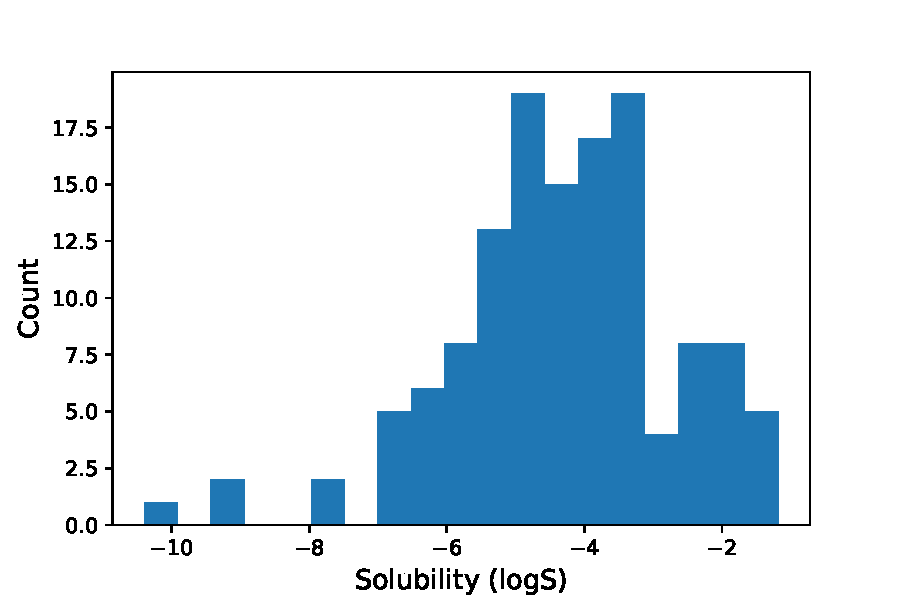
\includegraphics[width=\linewidth]{figures/histogram_solchal2_true_logs.pdf}
        \caption{SC2 solubility distribution, bin width of 0.5.}
    \end{subfigure}%
    \hfill
    \begin{subfigure}[t]{0.48\textwidth}
        \centering
        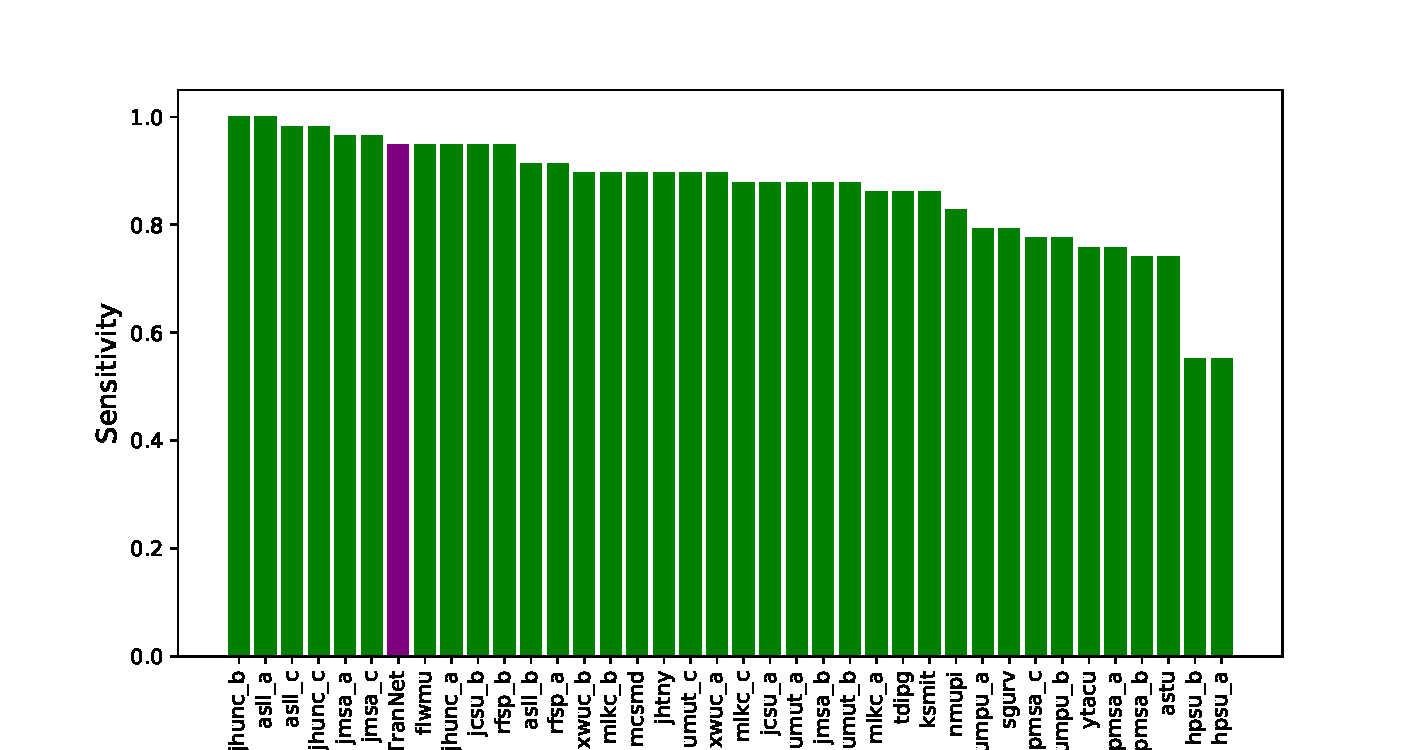
\includegraphics[width=\linewidth]{figures/hit_-4_solchal2.pdf}
        \caption{SC2 Sensitivity analysis. SolTranNet is shown in purple.}
    \end{subfigure}
    
    \begin{subfigure}[t]{0.32\textwidth}
        \centering
        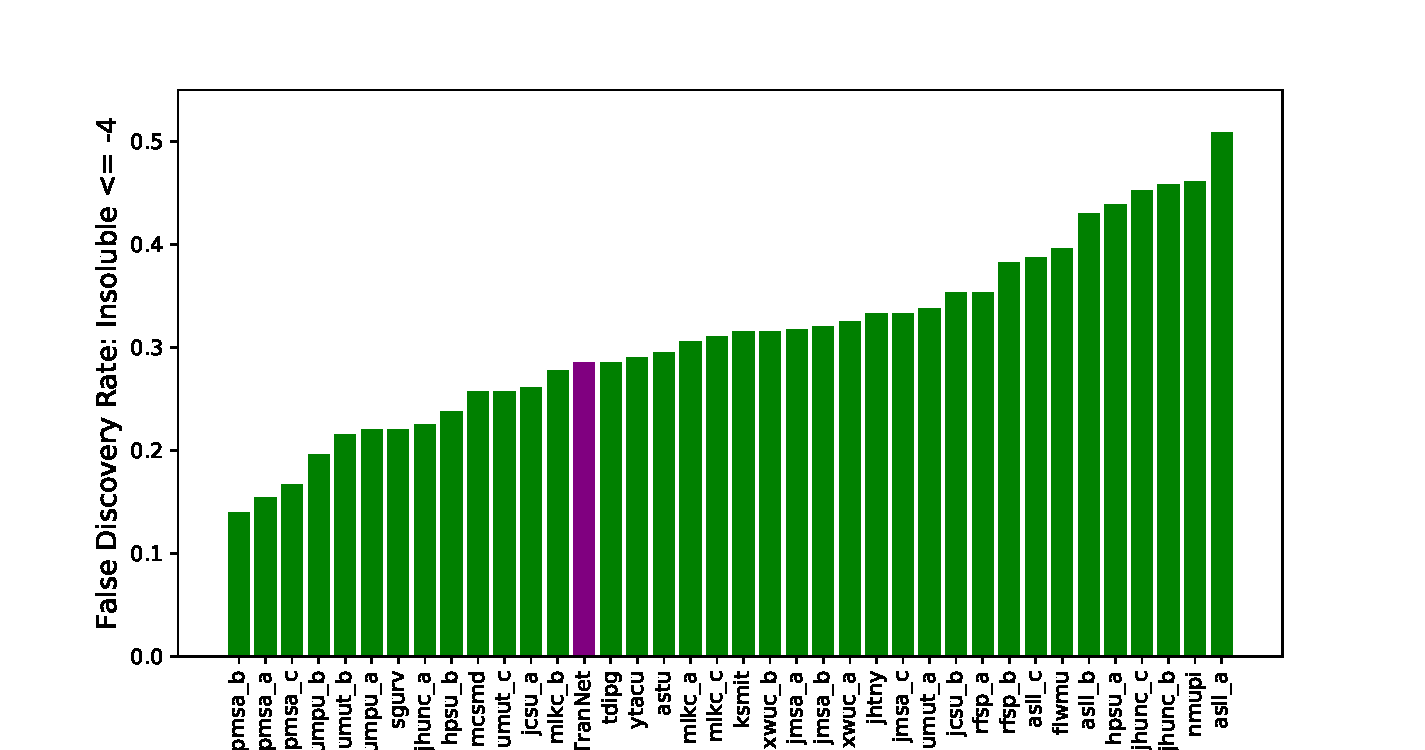
\includegraphics[width=\linewidth]{figures/fail_-4_solchal2.pdf}
        \caption{False discovery rates where insoluble is $LogS <=-4$. SolTranNet is shown in purple.}
    \end{subfigure}%
    \hfill
    \begin{subfigure}[t]{0.32\textwidth}
        \centering
        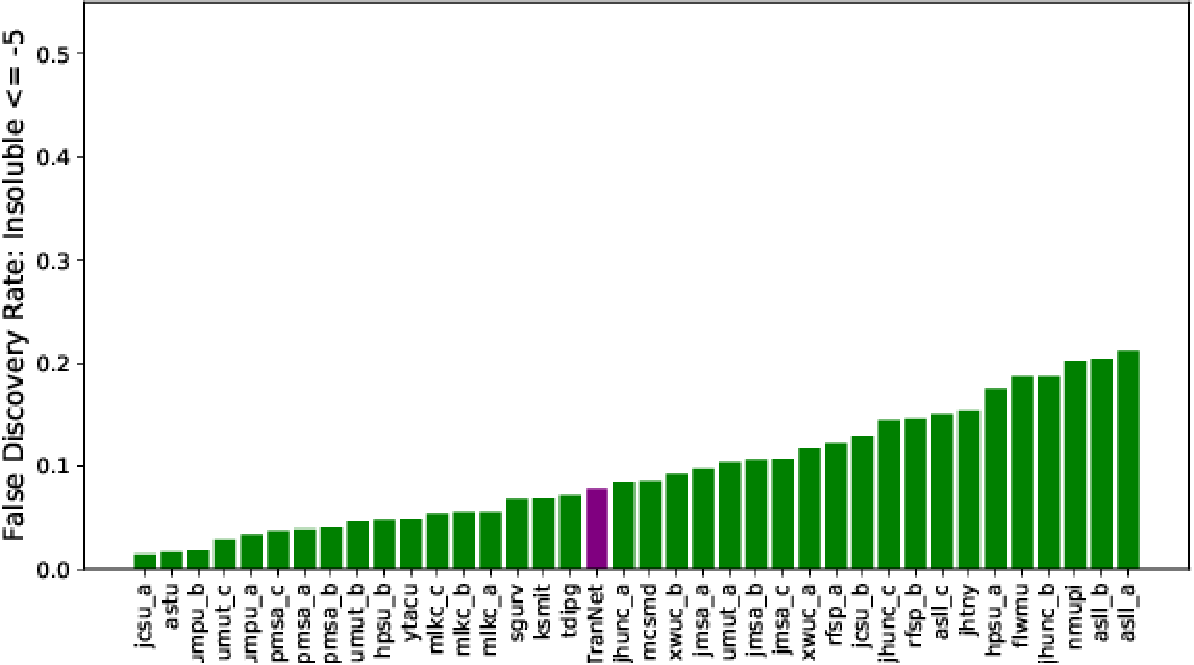
\includegraphics[width=\linewidth]{figures/fail_-5_solchal2.pdf}
        \caption{False discovery rates where insoluble is $LogS <=-5$. SolTranNet is shown in purple.}
    \end{subfigure}
    \hfill
    \begin{subfigure}[t]{0.32\textwidth}
        \centering
        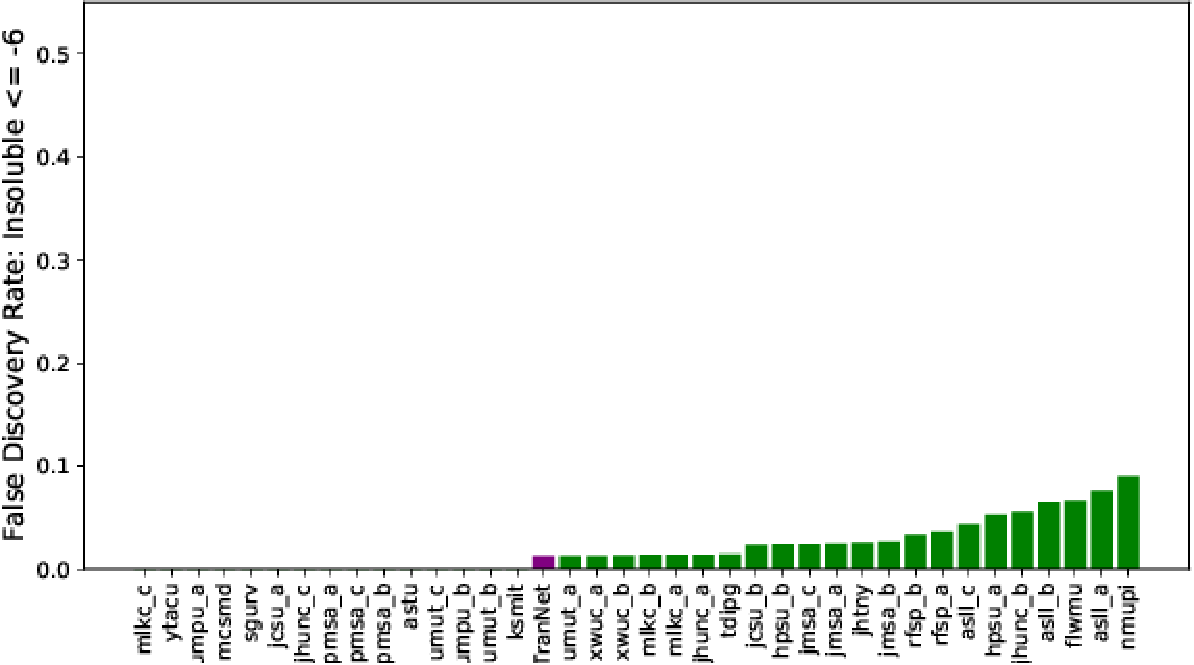
\includegraphics[width=\linewidth]{figures/fail_-6_solchal2.pdf}
        \caption{False discovery rates where insoluble is $LogS <=-6$. SolTranNet is shown in purple.}
    \end{subfigure}
    \caption{Recontextualizing the SC2 data. (a) Distribution of both SC2 test sets. We classified solubility as a molecule is soluble if its logS $> -4$. We then calculated the sensitivity (b) and false discovery rates (c-e). SolTranNet performs near state of the art in terms of sensitivity (94.8\%) and false discovery rate (1.30\% in e).}
    \label{fig:sc2redo}
\end{figure}

%%%%%%%%%%%%%%%%%%%%%%%%%%%%%%%%%%%%%%%%%%%%%%%%%%%%%%%%%%%%%%%%%%%%%
%% Discussion
%%%%%%%%%%%%%%%%%%%%%%%%%%%%%%%%%%%%%%%%%%%%%%%%%%%%%%%%%%%%%%%%%%%%%
\section{Discussion}

We described SolTranNet and evaluated it on a variety of datasets.
During model optimization we show that SolTranNet outperforms linear ML approaches (Table~\ref{tab:solsearchrmse}), and is competitive with other ML methods (Table~\ref{tab:othersetsrmse} and Fig~\ref{fig:sc2redo}).
Of particular note, we observe that smaller ML models perform better than their larger counterparts (Table~\ref{tab:solsearchrmse}).
This goes contrary to the observations of \citet{cui} where deeper models performed better.
Yet SolTranNet's best performing model with the same training and testing data achieved better performance than their 20-layer ResNet architecture \cite{cui} (Table~\ref{tab:othersetsrmse}).
We suspect this effect is due to the small training set.

The available solubility data is quite small, with ``large datasets'' being thousands of data points.
Small training set size makes it easier for ML methods to overfit their training data, and limits their generalization.
We observed this phenomenon with our larger models during our hyperparameter sweep (Table~\ref{tab:solsearchrmse}).
This is why we selected our final architecture by its performance on our withheld test set, and why models with dropout tended to perform better as both of these techniques help to reduce overfitting to the training set.
We hypothesize that the smaller models are more suited to solubility prediction until more training data becomes available.
Data augmentation is a potential approach to expand the available data, but we leave this to future work.

Another concern is the small size of the testing sets used in the community.
With test sets in the low hundreds of molecules, there is a limit on the power of conclusions we can draw about model performance.
Even when training on several thousand molecules, we observe worse performance when test set distributions are substantially different from the training set (Figure~\ref{fig:solhists}, Fold1 column Table\ref{tab:solsearchrmse}).
This indicates that our models are not learning generalizable molecular features to make their predictions.
The large range of the possible values in AqSolDB (14 log units) makes it easier to achieve high correlation statistics, which is why we favored analysis of the RMSE of the given predictions to compare model performance.

SolTranNet had worse performance on the SC2 dataset than the best performing group (Table~\ref{tab:othersetsrmse}).
However, it should be noted that the test sets for SC2 were not blind.
Thus the most relevant comparison to the reported metrics is the STN Best model in Table~\ref{tab:othersetsrmse}, as it is selected with knowledge of performance on the test set.
SolTranNet exhibited the largest amount of training variability on these test sets, which indicates that we could potentially increase performance by optimizing the SolTranNet architecture for these test sets.
Even the best reported models have an RMSE over half a log unit, which raises the question "What level of performance makes a model useful for drug discovery?"

We restructured the evaluation into a classification task to investigate this. 
We chose to analyze the sensitivity and false discovery rate, as we desire a model that correctly identifies soluble compounds (high sensitivity) and avoids falsely identifying insoluble compounds (low false discovery rate).
SolTranNet achieves comparable classification performance to the other methods submitted to SC2 (Figure~\ref{fig:sc2redo}).

We have shown that SolTranNet is capable of predicting aqueous solubility and outperforms linear ML approaches.
During our hyperparameter optimization, we demonstrate that models with more parameters do not perform better in our scaffold-based CCV splits and exhibit worse performance on a withheld test set (Table~\ref{tab:solsearchrmse},\ref{tab:solsearchr2}).
SolTranNet's smaller size, removal of the distance matrix, and implementation of multiprocessing makes it run 118 times faster than the original MAT implementation (Table:\ref{tab:timings}).
SolTranNet has comparable performance to current ML models (Tables~\ref{tab:othersetsrmse} and \ref{tab:othersetsr2}, Figure~\ref{fig:sc2redo}).
We have deployed SolTranNet via \textsc{pip} for easy integration into drug discovery pipelines, and its source code is available under an Apache open source license at \url{https://github.com/gnina/SolTranNet}.

%%%%%%%%%%%%%%%%%%%%%%%%%%%%%%%%%%%%%%%%%%%%%%%%%%%%%%%%%%%%%%%%%%%%%
%% The "Acknowledgement" section can be given in all manuscript
%% classes.  This should be given within the "acknowledgement"
%% environment, which will make the correct section or running title.
%%%%%%%%%%%%%%%%%%%%%%%%%%%%%%%%%%%%%%%%%%%%%%%%%%%%%%%%%%%%%%%%%%%%%
\begin{acknowledgement}

We thank Andrew McNutt and Jonathan King for their contributions during manuscript preparation.

\subsection{Data and Software}
SolTranNet is open source and available under the Apache2.0 license. SolTranNet is available via \textsc{pip} installation for \textsc{python3}, and the source code is available at \url{https://github.com/gnina/SolTranNet}. All datasets and code used for the analysis in this paper is available at \url{https://github.com/francoep/SolTranNet_paper}

\subsection{Funding Sources}
This work is supported by R01GM108340 from the National Institute of General Medical Sciences and a GPU donation from the NVIDIA corporation.

\end{acknowledgement}

%%%%%%%%%%%%%%%%%%%%%%%%%%%%%%%%%%%%%%%%%%%%%%%%%%%%%%%%%%%%%%%%%%%%%
%% The same is true for Supporting Information, which should use the
%% suppinfo environment.
%%%%%%%%%%%%%%%%%%%%%%%%%%%%%%%%%%%%%%%%%%%%%%%%%%%%%%%%%%%%%%%%%%%%%
\begin{suppinfo}

%This will usually read something like: ``Experimental procedures and
%characterization data for all new compounds. The class will
%automatically add a sentence pointing to the information on-line:
Supporting Information Available: Supplementary Figures~\ref{tab:wandsweep}-\ref{fig:saltfragr2} and Tables~\ref{tab:solsearchr2}-\ref{tab:othersetsr2}.
\end{suppinfo}

%%%%%%%%%%%%%%%%%%%%%%%%%%%%%%%%%%%%%%%%%%%%%%%%%%%%%%%%%%%%%%%%%%%%%
%% The appropriate \bibliography command should be placed here.
%% Notice that the class file automatically sets \bibliographystyle
%% and also names the section correctly.
%%%%%%%%%%%%%%%%%%%%%%%%%%%%%%%%%%%%%%%%%%%%%%%%%%%%%%%%%%%%%%%%%%%%%
\bibliography{references}
\end{document}